% ---------------------------------------------------------------------------
% Results section for the contact-model-aware selective-passivation PoC.
% Requires: \usepackage{graphicx}, \usepackage{booktabs}, \usepackage{amsmath}
% Figures live in figs/ (vector PDF); the summary table is table_summary.tex.
% All quantitative values are produced by paper/make_figures.py from the
% CURRENT robust (iteration-2) experiment logs in results_passivation_iter2/
% — regenerate the dataset with
%   python -m mujoco_sliding.experiments --all --sweep --governor-compare
% and the figures/table with `python paper/make_figures.py`.
% ---------------------------------------------------------------------------

% Narrow-figure width: defaults to \columnwidth (two-column layouts); a
% single-column wrapper may predefine \figwidth (see main.tex).
\providecommand{\figwidth}{\columnwidth}

\section{Results}
\label{sec:results}

Fig.~\ref{fig:overview} summarizes the experimental system and the
implemented pipeline. All experiments share the task of
Sec.~\ref{sec:task}\footnote{Adjust this reference to your setup section.}
($F_n^d = 5$~N, $v_t^d = 0.05$~m/s), the ledger parameters, and the robust
QP rows; only the task-contact predictor, the scripted human wrench, and
the controller mode vary between tests. All results in this section come
from one coherent dataset generated by the current robust implementation:
the ledger rows constrain the robust lower power estimate
$p^{\mathrm{pred}}_i(u) - \|\mathbf{w}_i\|\,\bar e_v$ under the configured
one-step velocity prediction-error bound $\bar e_v = 0.025$~m/s, so every
floor guarantee below is conditional on that bound --- which is itself
monitored: the largest error measured across all runs is $0.0115$~m/s
(peak utilization $0.46$) with zero violations. The comparison modes are
C0 (nominal), C1 (whole-port QP), C2 (residual QP), C3 (dual-ledger
task-weighted QP), and C4 (dual-ledger \emph{safe-anchor scalar}: the
command is restricted to the line from a feasible minimum-norm safety
anchor toward the nominal command, under the identical constraint rows).
Table~\ref{tab:summary} collects the summary metrics of every mode--test
combination. Across all runs the QP solves in $24$--$44~\mu$s (median)
with a worst 99th percentile of $57~\mu$s, well within the 1~kHz control
budget.

\begin{figure*}[t]
  \centering
  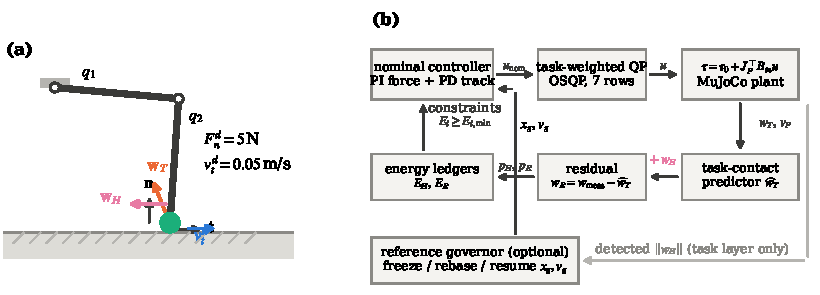
\includegraphics[width=\textwidth]{figs/fig1_overview.pdf}
  \caption{System and signal overview. (a)~Planar two-link robot with the
  spherical contact pad sliding on a horizontal surface; the task-contact
  wrench $\mathbf{w}_T$ and the scripted human wrench $\mathbf{w}_H$ act at
  the end-effector, and $(\mathbf{t},\mathbf{n})$ span the command plane.
  (b)~Implemented pipeline: the task-contact predictor
  $\widehat{\mathbf{w}}_T$ removes model-consistent contact wrench from the
  measurement, the residual $\mathbf{w}_R$ and human $\mathbf{w}_H$ ports
  feed the nested energy ledgers, and the task-weighted QP filters the
  nominal command subject to the robust ledger, human-power, torque, and
  torque-rate rows. The optional reference governor shapes only the nominal
  tangential reference and does not enter the certificate.}
  \label{fig:overview}
\end{figure*}

\subsection{False depletion under nominal sliding (Test A)}
\label{sec:res-a}

Fig.~\ref{fig:false-depletion} shows Test~A (oracle predictor, no human).
C0, C2, and C3 are indistinguishable: $\mathrm{RMSE}(F_n)\approx0.033$~N,
$\mathrm{RMSE}(v_t)\approx0.0025$~m/s, C3 within $0.02\,\%$ of C0, and the
C3 filter modifies the command on only $0.008\,\%$ of in-contact steps,
with both of its ledgers exactly constant (drift $\leq10^{-9}$~J). The
whole-port baseline C1, in contrast, charges the ordinary sliding-friction
dissipation ($\approx0.075$~W) to its protected ledger: $E_W$ drains and
triggers intervention at $t\approx5.9$~s. Because the whole-port force is
dominated by the (noisy, one-step-delayed) raw contact sample, riding that
ledger's floor is not solver-feasible in this plant: 7658 steps fall back
to the bounded emergency action, which stalls tangential sliding while
holding the normal push --- the pad keeps regulating $F_n\approx5$~N
(Fig.~\ref{fig:false-depletion}b) but the sliding task is permanently
halted (Fig.~\ref{fig:false-depletion}c). This is the false-passivation
failure mode that motivates contact-model subtraction: an accurate task
model leaves the nominal task untouched, whereas whole-port accounting
destroys the tangential task on friction alone and cannot even ride its
own floor cleanly (claims~1--2).

\begin{figure}[t]
  \centering
  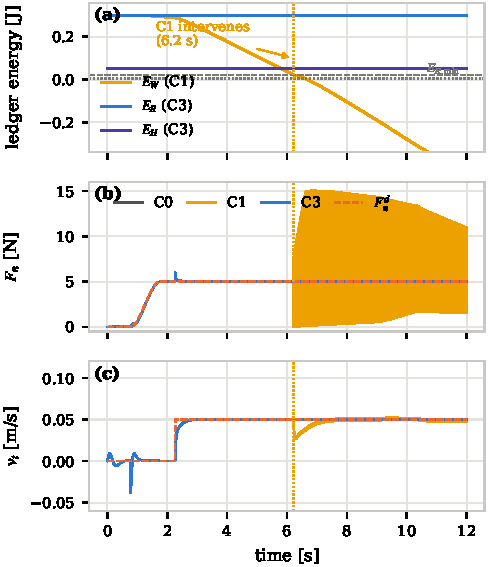
\includegraphics[width=\figwidth]{figs/fig2_false_depletion.pdf}
  \caption{Test~A (oracle model, no human): false depletion under nominal
  sliding. (a)~The whole-port ledger $E_W$ of C1 drains on ordinary task
  friction and triggers intervention at $5.9$~s (vertical line), while the
  C3 residual and human ledgers remain exactly at their initial values.
  (b)~Normal force and (c)~tangential velocity: C0 and C3 overlap; C1
  stalls the sliding task permanently (via its bounded fallback, which
  preserves the normal push but marks the run solver-infeasible).}
  \label{fig:false-depletion}
\end{figure}

\subsection{Model mismatch stays in the residual port (Test B)}
\label{sec:res-b}

With the regularized friction predictor at $\widehat{\mu}=0.20$ (true
$\mu\approx0.30$) and no human, the mismatch power
$p_\Delta\approx-(\mu-\widehat{\mu})F_n v_t\approx-25$~mW discharges only
the residual ledger (Fig.~\ref{fig:mismatch}): $E_H$ stays exactly at
$0.05$~J (drift $\leq10^{-9}$~J) while $E_R$ bleeds from $0.30$~J to
$0.023$~J over the 15-s run. The first ledger-driven intervention
consequently moves from $5.95$~s (whole-port C1) to $14.59$~s (residual,
C3): the predictor postpones passivation until \emph{unexplained} contact
power has consumed the residual budget, rather than total task friction
(claim~3). The attribution identities hold to machine precision throughout
($\mathbf{w}_R=\mathbf{w}_\Delta$ here; $p_R = p_H + p_\Delta$ in every
test).

\begin{figure}[t]
  \centering
  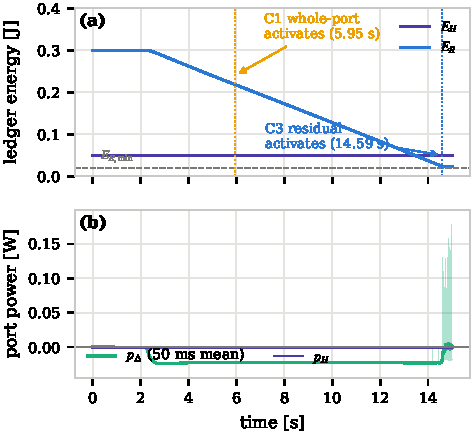
\includegraphics[width=\figwidth]{figs/fig3_mismatch_residual.pdf}
  \caption{Test~B (friction mismatch $\widehat{\mu}=0.20$, no human).
  (a)~The human ledger is exactly constant while the residual ledger
  depletes; first ledger-driven interventions of C1 ($5.95$~s) and C3
  ($14.59$~s) are marked. (b)~Port powers: the depletion is carried
  entirely by the mismatch power $p_\Delta$ while $p_H\equiv0$.}
  \label{fig:mismatch}
\end{figure}

\subsection{Human-directed power and energy limiting (Test C)}
\label{sec:res-c}

Fig.~\ref{fig:human-limiting} is the central quantitative comparison. The
nominal controller (C0) works against the $3$-N blocking human at
$-p_H\approx0.15$~W for the entire hold and delivers $0.361$~J. C2
(residual ledger only) behaves almost identically until its large residual
budget is exhausted: the peak human-directed power is unchanged
($0.1499$~W) and $0.278$~J are extracted, because nothing in C2
distinguishes the human from generic unexplained contact. C3 clips the
instantaneous power at the $P_H^{\max}=0.10$~W row (measured peak
$0.0997$~W), lets the CBF row park $E_H$ just above its floor (run minimum
$0.0064$~J $>E_{H,\min}=0.005$~J), and saturates the cumulative output at
$0.044$~J against the $0.045$-J budget --- an $8.3\times$ reduction over C0
enforced by the small dedicated ledger rather than by tuning (claim~4).
After release the robot recovers nominal sliding in $0.66$~s.

\begin{figure}[t]
  \centering
  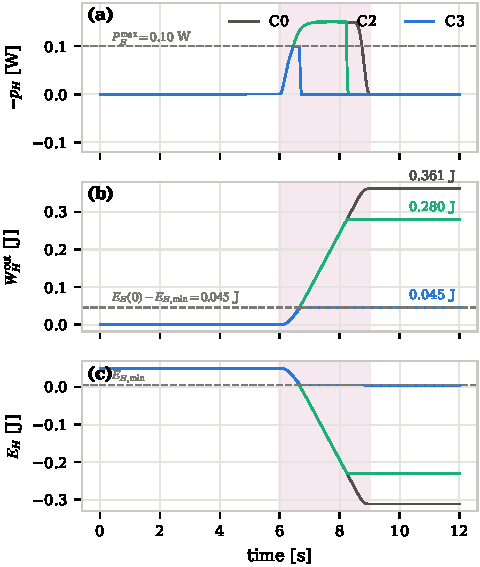
\includegraphics[width=\figwidth]{figs/fig4_human_limiting.pdf}
  \caption{Test~C (oracle model, $3$-N blocking human, shaded window):
  human-port limiting across C0/C2/C3. (a)~Instantaneous extracted power
  $-p_H$ with the $0.10$-W row; (b)~cumulative human-directed energy
  $W_H^{\mathrm{out}}$ against the $0.045$-J budget; (c)~the human ledger:
  C3 stays above $E_{H,\min}$, while the (unconstrained, observed) ledgers
  of C0 and C2 run far below it.}
  \label{fig:human-limiting}
\end{figure}

\subsection{Combined mismatch and human interaction (Test D)}
\label{sec:res-d}

Test~D repeats the blocking profile under $\widehat{\mu}=0.20$
(Fig.~\ref{fig:combined}). The human ledger reproduces Test~C
($E_H\geq0.0064$~J, peak $0.0997$~W), while the residual ledger now pays
for both channels and reaches $0.041$~J: the stacked decomposition in
Fig.~\ref{fig:combined}b shows $-p_R$ separating into the human share
$-p_H$ (bounded by the human rows) and the persistent mismatch share
$-p_\Delta$. The nested ledgers therefore attribute energy to the correct
ports simultaneously. As a diagnostic of the dedicated human ledger's
value: C2 in this same scenario exhausts $E_R$ through the combined drain
and logs 1192 solver-infeasible steps around the release, whereas C3 ---
whose human rows yield first --- never lets $E_R$ within $0.02$~J of its
floor and stays feasible on every step.

\begin{figure}[t]
  \centering
  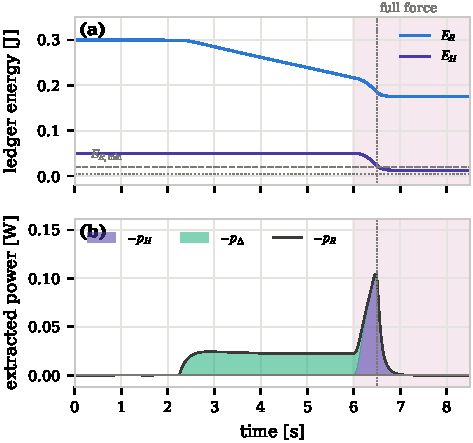
\includegraphics[width=\figwidth]{figs/fig5_combined_decomposition.pdf}
  \caption{Test~D (mismatch $\widehat{\mu}=0.20$ plus blocking human).
  (a)~Both ledgers respond: $E_H$ tracks only human power, $E_R$ tracks
  human plus mismatch. (b)~Extracted-power decomposition
  $-p_R=-p_H-p_\Delta$ (50-ms means; stacked areas sum to the black
  $-p_R$ trace).}
  \label{fig:combined}
\end{figure}

\subsection{Filter-level task allocation under oblique interaction
(Test E1)}
\label{sec:res-e1}

Test~E1 is a \emph{filter-only allocation ablation}: given the same
governor-off nominal controller (the reference governor is disabled for
both runs) and the same robust human-energy, residual-energy, human-power,
torque, and torque-rate rows, does the full two-dimensional task-weighted
QP (C3) preserve the normal-force task better than the safe-anchor scalar
restriction (C4)? The oblique human force
$\mathbf{w}_H=\tfrac{3}{\sqrt2}(-\mathbf{t}-\mathbf{n})$~N is applied with
the standard cosine profile, and E1 is evaluated \emph{only} on the
full-magnitude plateau
$[t_{\mathrm{start}}+t_{\mathrm{rise}},\,
t_{\mathrm{start}}+t_{\mathrm{rise}}+t_{\mathrm{hold}}] = [6.5, 8.5]$~s
(derived from the scenario configuration): the force-removal transient and
the post-release recovery are excluded \emph{by design}, because E1
isolates the geometry of the command filter, not recovery behavior ---
recovery under a moving reference is governed by the tracking debt the
reference accumulates and is treated separately by the reference-governor
ablation of Sec.~\ref{sec:res-governor}. Only metrics and plots are
clipped to this window; the simulations, logs, and all certificate
quantities use the complete 12-s runs.

Both controllers satisfy the identical certificate on the full run (zero
infeasible, emergency, prediction-bound, and floor violations;
$E_H\geq0.0064$~J, $E_R\geq0.256$~J, peak $-p_H=0.092$~W for both). Within
the E1 window their \emph{tangential} behavior is nearly identical --- the
filtered tangential commands differ by only $0.077$~N RMS ($0.195$~N
maximum) against a $\sim23$-N tangential safety action, and
$\mathrm{RMSE}(v_t)$ agrees to $2\,\%$ ($0.0457$ vs.\ $0.0465$~m/s) ---
because the same active human-energy boundary largely determines the
tangential safety action in both filters. The allocation of the
\emph{normal} command is where they part: C3 preserves the normal command
more closely (RMS deviation from nominal $0.35$~N, vs.\ $3.91$~N for C4;
the two filters' normal commands differ by $2.76$~N RMS, $3.41$~N
maximum), and the normal-force cost follows directly:
%
\begin{equation}
\mathrm{rmse}_{F_n}^{\mathrm{E1}} = 0.512~\mathrm{N}\ \text{(C3)}
\qquad\text{vs.}\qquad
2.264~\mathrm{N}\ \text{(C4)},
\end{equation}
%
a $4.4\times$ difference (C0 reference: $0.112$~N). C4's scalar
interpolation from the safety anchor toward nominal cannot trade the two
axes independently, so satisfying the human rows drags its normal command
away from the force task (Fig.~\ref{fig:qp-vs-scalar}c) and $F_n$ sags
toward $2.3$~N, while C3 spends the entire intervention in the tangential
axis (claim~5).

\begin{figure*}[t]
  \centering
  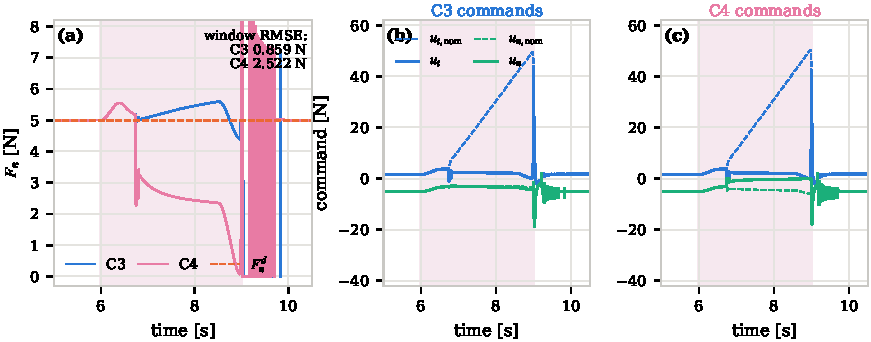
\includegraphics[width=\textwidth]{figs/fig6_qp_vs_scalar.pdf}
  \caption{Test E1, evaluated over the full-magnitude oblique-interaction
  plateau ($6.5$--$8.5$~s, shaded; the lighter band is the force-rise
  context). Both controllers use the same governor-off nominal reference
  and the same robust passivity rows; force removal and post-release
  recovery are excluded by design. (a)~Normal-force regulation with the
  freshly computed E1-window RMSE. (b)~C3 commands: the intervention is
  carried almost entirely by the tangential axis while the normal command
  stays close to its nominal. (c)~C4 commands: the safe-anchor scalar
  moves both axes along one line, pulling the normal command off the force
  task. The full-dimensional C3 QP produces nearly the same tangential
  safety action as C4 ($0.08$~N RMS difference) while preserving the
  normal-force task more closely than the safe-anchor scalar restriction.}
  \label{fig:qp-vs-scalar}
\end{figure*}

\subsection{Ledger charging, capping, and discharge (Test F)}
\label{sec:res-f}

Fig.~\ref{fig:charge} traces the human ledger through a helping
($+3$~N$\,\mathbf{t}$) followed by a blocking ($-3$~N$\,\mathbf{t}$)
pulse. During helping, $p_H>0$ charges $E_H$ from $0.05$~J to the
$0.08$-J cap, where charging saturates (discharge is never clamped, so the
cap is the only nonlinearity). The later blocking pulse first spends the
stored credit --- the robot resists longer than in Test~C --- and then
approaches the floor (minimum $0.0064$~J) with the extraction again
power-limited at $0.10$~W. Energy received from the human genuinely
extends the budget for later interaction, while the cap bounds how much
history may accumulate.

\begin{figure}[t]
  \centering
  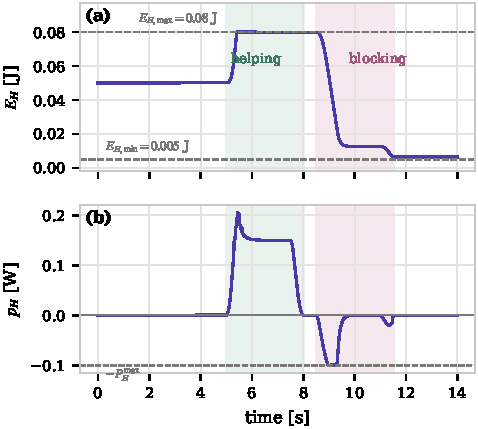
\includegraphics[width=\figwidth]{figs/fig7_charge_discharge.pdf}
  \caption{Test~F (helping then blocking; green/pink windows).
  (a)~$E_H$ charges to the $0.08$-J cap, plateaus, and later discharges
  toward the floor. (b)~The human-port power showing the charge ($p_H>0$)
  and bounded discharge ($p_H\geq-0.10$~W) phases.}
  \label{fig:charge}
\end{figure}

\subsection{Reference-governor ablation}
\label{sec:res-governor}

A time-indexed moving reference keeps advancing while the passivity filter
holds the robot, accumulating tracking debt; on release, that debt is
repaid as a catch-up burst. Fig.~\ref{fig:governor} compares C3 with the
governor disabled and enabled on the blocking scenario: the burst reaches
$0.68$~m/s and a $24.2$-N normal-force transient without the governor
(peaking during the force ramp-out; still $11.6$~N after the force has
fully vanished), versus $0.050$~m/s and $5.1$~N with it --- the
post-release $F_n$ overshoot is reduced by $98.6\,\%$ and the velocity
stays within $0.2\,\%$ of $v_t^d$. Panel~(c)
shows the mechanism: the governed reference freezes and continuously
rebases onto the end-effector during the interaction (even following the
human's back-push), then resumes with a cosine ramp from the rebased
position; both position and velocity references remain continuous. The
certificate quantities are unaffected by construction (the governed run
keeps $E_H\geq E_{H,\min}$ with a peak extraction of only $0.010$~W,
since yielding removes the incentive to fight the human). The governor is
purely a task/recovery policy (claim~6); it is disabled in the certificate
tests A--F above so the ledger rows are genuinely exercised, and in any
end-to-end behavioral comparison the \emph{same} governor must be applied
to C3 and C4 alike --- which is why E1 excludes release behavior rather
than letting an ungoverned catch-up transient contaminate a filter-level
comparison.

\begin{figure}[t]
  \centering
  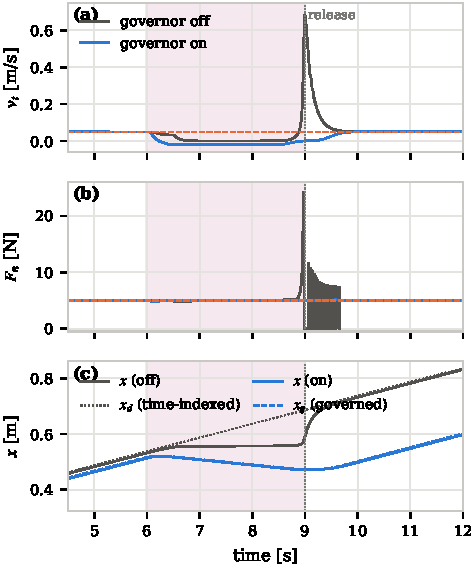
\includegraphics[width=\figwidth]{figs/fig8_governor.pdf}
  \caption{Reference-governor ablation (blocking scenario, C3; release
  marked at $9$~s). (a)~Tangential velocity: the $0.68$-m/s catch-up burst
  is replaced by a ramp bounded by $v_t^d$. (b)~Normal force: the release
  transient is suppressed from a $24.2$-N peak (reached during the force
  ramp-out) to $5.1$~N. (c)~References:
  the governed $x_g$ freezes and rebases onto the end-effector during the
  interaction instead of tracking the time-indexed $x_d$.}
  \label{fig:governor}
\end{figure}

\subsection{Friction-model sweep}
\label{sec:res-sweep}

Fig.~\ref{fig:sweep} sweeps the predictor coefficient
$\widehat{\mu}\in\{0.20,0.25,0.30,0.35\}$ for C3. Residual depletion
scales monotonically with the model error: $\widehat{\mu}=0.20$ reaches
the floor region ($E_R\to0.023$~J), $0.25$ consumes roughly half the
budget, and $\widehat{\mu}\geq0.30$ produces no mismatch-driven depletion
at all --- those predictors only \emph{charge} the ledger (the plant's
regularized effective friction sits slightly below the nominal
$\mu=0.30$, so their $p_\Delta\geq0$ while sliding). With a blocking human
the first intervention is dominated by the human rows and is therefore
independent of $\widehat{\mu}$ ($6.45$~s), while without a human it occurs
only for the largest mismatch ($14.59$~s at $\widehat{\mu}=0.20$). With
the human present, task tracking is exactly flat across the sweep; without
the human it is flat except at $\widehat{\mu}=0.20$, whose elevated RMSE
stems entirely from the brief post-intervention stall after $14.59$~s
rather than from degraded sliding before it --- moderate model error costs
residual budget, not task performance. The human-ledger floor is respected
at every $\widehat{\mu}$.

\begin{figure*}[t]
  \centering
  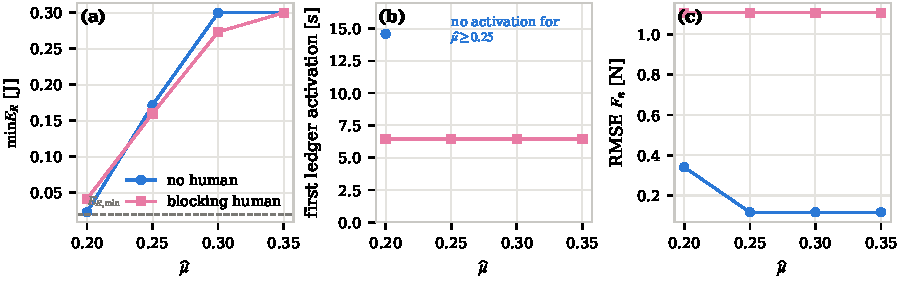
\includegraphics[width=\textwidth]{figs/fig9_sweep.pdf}
  \caption{Friction-predictor sweep for C3 with and without the blocking
  human. (a)~Minimum residual-ledger level: mismatch-driven depletion
  scales with $|\mu-\widehat{\mu}|$ and vanishes for
  $\widehat{\mu}\geq0.30$ (the blocking-human family still discharges
  through the human share of $p_R$). (b)~First ledger-driven intervention:
  human-driven ($6.45$~s) when present, mismatch-driven ($14.59$~s at
  $\widehat{\mu}=0.20$) or absent otherwise. (c)~Sliding-phase
  $\mathrm{RMSE}(F_n)$: flat with the human at every $\widehat{\mu}$; the
  no-human point at $\widehat{\mu}=0.20$ is elevated only by the brief
  post-intervention stall.}
  \label{fig:sweep}
\end{figure*}

% Table I (double-column float; input kept separate for editing)
\begin{table*}[t]
\centering
\caption{Summary metrics for all controller modes and tests (current robust implementation). RMSE values are over the sliding phase, EXCEPT the Test E1 rows (marked $^{\dagger}$), which report $\mathrm{rmse}_{F_n}^{\mathrm{E1}}$ and $\mathrm{rmse}_{v_t}^{\mathrm{E1}}$ over the full-force plateau $[t_{\mathrm{start}}+t_{\mathrm{rise}},\,t_{\mathrm{start}}+t_{\mathrm{rise}}+t_{\mathrm{hold}}]$ only, because E1 is a filter-allocation ablation that excludes the release transient by design; all other columns (peak power, energies, counts) always use the complete unclipped run. $-p_H^{\max}$ is the peak instantaneous power delivered to the human port; $W_H^{\mathrm{out}}$ is the maximum of the SIGNED cumulative human-directed output energy (net; in Test F the helping phase offsets the later extraction, so it stays at zero); $\min E_H$, $\min E_R$ are raw ledger minima (discharge is never clamped); ``act.'' is the fraction of in-contact steps on which the filter modified the command; $t_{\mathrm{act}}$ is the first ledger-driven intervention; ``fail'' counts QP solve failures handled by the bounded emergency fallback. Test S is the 32-s alternating helping/blocking certificate stress run (reference governor enabled).}
\label{tab:summary}
\small
\setlength{\tabcolsep}{4.5pt}
\begin{tabular}{llrrrrrrrrr}
\toprule
Test & Mode & RMSE $F_n$ & RMSE $v_t$ & $-p_H^{\max}$ & $W_H^{\mathrm{out}}$ & $\min E_H$ & $\min E_R$ & act. & $t_{\mathrm{act}}$ & fail \\
 & & [N] & [m/s] & [W] & [J] & [J] & [J] & [\%] & [s] & \\
\midrule
A & C0 & 0.033 & 0.0025 & 0.000 & 0.000 & 0.050 & 0.300 & 0.00 & -- & 0 \\
A & C1 & 0.424 & 0.0400 & 0.000 & 0.000 & 0.050 & 0.300 & 58.94 & 5.95 & 7658 \\
A & C2 & 0.033 & 0.0025 & 0.000 & 0.000 & 0.050 & 0.300 & 0.01 & -- & 0 \\
A & C3 & 0.033 & 0.0025 & 0.000 & 0.000 & 0.050 & 0.300 & 0.01 & -- & 0 \\
A & C4 & 0.033 & 0.0025 & 0.000 & 0.000 & 0.050 & 0.300 & 0.01 & -- & 0 \\
\addlinespace[2pt]
B & C0 & 0.117 & 0.0025 & 0.000 & 0.000 & 0.050 & 0.014 & 0.00 & -- & 0 \\
B & C1 & 0.407 & 0.0409 & 0.000 & 0.000 & 0.050 & 0.218 & 61.82 & 5.95 & 8658 \\
B & C2 & 0.341 & 0.0030 & 0.000 & 0.000 & 0.050 & 0.023 & 1.13 & 14.59 & 0 \\
B & C3 & 0.341 & 0.0030 & 0.000 & 0.000 & 0.050 & 0.023 & 1.13 & 14.59 & 0 \\
\addlinespace[2pt]
C & C0 & 0.219 & 0.0051 & 0.150 & 0.361 & -0.311 & -0.061 & 0.00 & -- & 0 \\
C & C2 & 0.543 & 0.0242 & 0.150 & 0.278 & -0.228 & 0.022 & 7.63 & 8.09 & 0 \\
C & C3 & 1.108 & 0.0694 & 0.100 & 0.044 & 0.006 & 0.256 & 22.40 & 6.45 & 0 \\
C & C4 & 2.215 & 0.0690 & 0.100 & 0.044 & 0.006 & 0.256 & 22.42 & 6.45 & 0 \\
\addlinespace[2pt]
D & C0 & 0.219 & 0.0051 & 0.150 & 0.361 & -0.311 & -0.276 & 0.00 & -- & 0 \\
D & C2 & 1.421 & 0.0445 & 0.150 & 0.189 & -0.139 & 0.019 & 28.75 & 7.37 & 1192 \\
D & C3 & 1.108 & 0.0694 & 0.100 & 0.044 & 0.006 & 0.041 & 22.40 & 6.45 & 0 \\
D & C4 & 2.215 & 0.0690 & 0.100 & 0.044 & 0.006 & 0.049 & 22.42 & 6.45 & 0 \\
\addlinespace[2pt]
E$^{\dagger}$ & C0 & 0.112 & 0.0021 & 0.107 & 0.259 & -0.209 & 0.041 & 0.00 & -- & 0 \\
E$^{\dagger}$ & C3 & 0.512 & 0.0457 & 0.092 & 0.044 & 0.006 & 0.256 & 21.12 & 6.59 & 0 \\
E$^{\dagger}$ & C4 & 2.264 & 0.0465 & 0.092 & 0.044 & 0.006 & 0.256 & 21.11 & 6.59 & 0 \\
\addlinespace[2pt]
F & C0 & 0.286 & 0.0061 & 0.150 & 0.000 & -0.281 & 0.139 & 0.00 & -- & 0 \\
F & C3 & 0.938 & 0.0571 & 0.100 & 0.000 & 0.006 & 0.300 & 19.01 & 8.95 & 0 \\
\addlinespace[2pt]
S & C3 & 0.044 & 0.0139 & 0.010 & 0.000 & 0.050 & 0.300 & 0.00 & -- & 0 \\
\bottomrule
\end{tabular}
\end{table*}


\subsection{Summary}
\label{sec:res-summary}

Table~\ref{tab:summary} condenses the comparison on the current robust
dataset. Whole-port accounting (C1) falsely consumes its budget on
predictable friction and permanently stalls the task it was meant to
protect (its floor cannot even be ridden solver-feasibly in this plant ---
7658 and 8658 bounded-fallback steps in Tests A and B, reported rather
than hidden); contact-model subtraction (C2/C3) postpones intervention
until the interaction is unexplained by the task model; the dedicated
human ledger and power row (C3) reduce peak and cumulative human-directed
output by factors of $1.5$ and $8.3$ relative to C0 while the residual
ledger absorbs model error (and keeps C3 feasible in Test~D, where C2
fails); the full task-weighted QP preserves normal-force regulation
$4.4\times$ better than the safe-anchor scalar over the E1 plateau while
producing an almost identical tangential safety action; and the reference
governor removes the post-release burst without touching any certificate
quantity. A 32-s stress run with six alternating helping/blocking pulses
sustains all of the above with zero infeasible steps, zero bound or floor
violations, and bit-exact ledger accounting throughout.
